\documentclass{bmcart}

%%% Load packages
%\usepackage{amsthm,amsmath}
\usepackage{amsmath}
\usepackage{setspace}
\usepackage{lineno}
\usepackage{url}
\linenumbers
\RequirePackage[sort]{natbib}
%\RequirePackage[authoryear]{natbib}% uncomment this for author-year bibliography
%\RequirePackage{hyperref}
\usepackage[utf8]{inputenc} %unicode support
%\usepackage[applemac]{inputenc} %applemac support if unicode package fails
%\usepackage[latin1]{inputenc} %UNIX support if unicode package fails
\usepackage{graphicx}
% \def\includegraphic{}
% \def\includegraphics{}


\startlocaldefs
\newcommand{\obs}{\mathbf{y}}
\newcommand{\cov}{\mathbf{x}}
\newcommand{\state}{z}
\newcommand{\dbic}{\ensuremath \Delta \textrm{BIC}}
\newcommand{\bmb}[1]{\textbf{[BMB: #1]}}
\endlocaldefs


%%% Begin ...
\begin{document}

%\setcounter{page}{0}  %% ugh, article template assumes starting on odd page!
% \newpage

%%% Start of article front matter
\begin{frontmatter}

\begin{fmbox}
\dochead{Research}

%% TO DO
% author references (maybe fix programmatically?)
% acknowledgments

%%%%%%%%%%%%%%%%%%%%%%%%%%%%%%%%%%%%%%%%%%%%%%
%%                                          %%
%% Enter the title of your article here     %%
%%                                          %%
%%%%%%%%%%%%%%%%%%%%%%%%%%%%%%%%%%%%%%%%%%%%%%

\title{Incorporating Periodic Variability in Hidden Markov Models for Animal Movement}

%%%%%%%%%%%%%%%%%%%%%%%%%%%%%%%%%%%%%%%%%%%%%%
%%                                          %%
%% Enter the authors here                   %%
%%                                          %%
%% Specify information, if available,       %%
%% in the form:                             %%
%%   <key>={<id1>,<id2>}                    %%
%%   <key>=                                 %%
%% Comment or delete the keys which are     %%
%% not used. Repeat \author command as much %%
%% as required.                             %%
%%                                          %%
%%%%%%%%%%%%%%%%%%%%%%%%%%%%%%%%%%%%%%%%%%%%%%

\author[
   addressref={aff1},                   % id's of addresses, e.g. {aff1,aff2}         
   email={lim88@mcmaster.ca}   % email address
]
{\inits{ML}\fnm{Michael} \snm{Li}}
\author[
   addressref={aff1,aff2},
   email={bolker@mcmaster.ca}
]{\inits{BMB}\fnm{Benjamin M.} \snm{Bolker}}

%%%%%%%%%%%%%%%%%%%%%%%%%%%%%%%%%%%%%%%%%%%%%%
%%                                          %%
%% Enter the authors' addresses here        %%
%%                                          %%
%% Repeat \address commands as much as      %%
%% required.                                %%
%%                                          %%
%%%%%%%%%%%%%%%%%%%%%%%%%%%%%%%%%%%%%%%%%%%%%%

\address[id=aff1]{                            % unique id
  \orgname{Department of Biology, McMaster University}, % university, etc
  \street{1280 Main St. West},                     %
  \postcode{L8S 4K1},                                % post or zip code
  \city{Hamilton, Ontario},                              % city
  \cny{Canada}                                    % country
}
\address[id=aff2]{
  \orgname{Department of Mathematics and Statistics, McMaster University},
  \street{1280 Main St. West},
  \postcode{L8S 4K1},
  \city{Hamilton, Ontario},
  \cny{Canada}
}

%%%%%%%%%%%%%%%%%%%%%%%%%%%%%%%%%%%%%%%%%%%%%%
%%                                          %%
%% Enter short notes here                   %%
%%                                          %%
%% Short notes will be after addresses      %%
%% on first page.                           %%
%%                                          %%
%%%%%%%%%%%%%%%%%%%%%%%%%%%%%%%%%%%%%%%%%%%%%%

\begin{artnotes}
% \note{Sample of title note}     % note to the article
% \note[id=n1]{Equal contributor} % note, connected to author
\end{artnotes}

\end{fmbox}% comment this for two column layout

%%%%%%%%%%%%%%%%%%%%%%%%%%%%%%%%%%%%%%%%%%%%%%
%%                                          %%
%% The Abstract begins here                 %%
%%                                          %%
%% Please refer to the Instructions for     %%
%% authors on http://www.biomedcentral.com  %%
%% and include the section headings         %%
%% accordingly for your article type.       %%
%%                                          %%
%%%%%%%%%%%%%%%%%%%%%%%%%%%%%%%%%%%%%%%%%%%%%%

\begin{abstractbox}

\begin{abstract} % abstract


%% need to break into background, 

% More generally, we point out that model misspecification
% (omitting important sources of variation) can lead to overfitting,
% and as a corollary that incorporating previously neglected
% structure in statistical models can allow more
% accurate assessment of appropriate model complexity.

\parttitle{Background} 
Clustering time-series data into discrete groups can improve 
prediction and provide insight into the nature of underlying,
unobservable states of the system. However, temporal variation in 
probabilities of group occupancy, or the rates at which individuals move between groups, can obscure
such signals. We use finite mixture and hidden Markov models (HMMs), two
standard clustering techniques, to model long-term hourly
movement data from Florida panthers (\emph{Puma concolor coryi}).
Allowing for temporal heterogeneity in transition probabilities, a straightforward 
but little-used extension of the standard HMM framework, 
resolves some shortcomings of current
models and clarifies the behavioural patterns of
panthers.

\parttitle{Results}

Simulations and analyses of panther data showed that model
misspecification (omitting important sources of variation) can lead to
overfitting/overestimating the underlying number of behavioural
states.  Models incorporating temporal heterogeneity identify fewer
underlying states, and can make out-of-sample predictions that
capture observed diurnal and autocorrelated movement patterns exhibited by
Florida panthers.

\parttitle{Conclusion}

Incorporating temporal heterogeneity improved goodness of fit and predictive
capability as well as
reducing the selected number of behavioural states 
to a more biologically interpretable level. Our results
suggest that incorporating additional structure in statistical models 
of movement behaviour can
allow more accurate assessment of appropriate model complexity.

\end{abstract}

%%%%%%%%%%%%%%%%%%%%%%%%%%%%%%%%%%%%%%%%%%%%%%
%%                                          %%
%% The keywords begin here                  %%
%%                                          %%
%% Put each keyword in separate \kwd{}.     %%
%%                                          %%
%%%%%%%%%%%%%%%%%%%%%%%%%%%%%%%%%%%%%%%%%%%%%%

\begin{keyword}
\kwd{Hidden Markov Model}
\kwd{Animal Movement}
\kwd{Temporal Autocorrelation}
\kwd{Temporal Heterogeneity}
\kwd{Florida Panther}
\end{keyword}

% MSC classifications codes, if any
%\begin{keyword}[class=AMS]
%\kwd[Primary ]{}
%\kwd{}
%\kwd[; secondary ]{}
%\end{keyword}

\end{abstractbox}
%
%\end{fmbox}% uncomment this for twcolumn layout

\end{frontmatter}

%%%%%%%%%%%%%%%%%%%%%%%%%%%%%%%%%%%%%%%%%%%%%%
%%                                          %%
%% The Main Body begins here                %%
%%                                          %%
%% Please refer to the instructions for     %%
%% authors on:                              %%
%% http://www.biomedcentral.com/info/authors%%
%% and include the section headings         %%
%% accordingly for your article type.       %%
%%                                          %%
%% See the Results and Discussion section   %%
%% for details on how to create sub-sections%%
%%                                          %%
%% use \cite{...} to cite references        %%
%%  \cite{koon} and                         %%
%%  \cite{oreg,khar,zvai,xjon,schn,pond}    %%
%%  \nocite{smith,marg,hunn,advi,koha,mouse}%%
%%                                          %%
%%%%%%%%%%%%%%%%%%%%%%%%%%%%%%%%%%%%%%%%%%%%%%

%%%%%%%%%%%%%%%%%%%%%%%%% start of article main body
% <put your article body there>

%%%%%%%%%%%%%%%%
%% Background %%
%%
% \section*{Content}
% Text and results for this section, as per the individual journal's instructions for authors. %\cite{koon,oreg,khar,zvai,xjon,schn,pond,smith,marg,hunn,advi,koha,mouse}

\doublespacing

\section*{Background}

Given a sequence of animal movements, movement models aim to find a parsimonious description
that can be used to understand past movements and predict
future movements. Ecologists have long considered the effects of
individual-level covariates (sex, age, nutritional status) and
environmental covariates (habitat type, location of predators or prey)
on movement \cite{patterson2008state, mckenzie2009first, pal1998dispersal}. 
More recently, modelers have developed
\emph{hidden Markov models} (HMMs)
\cite{firle_influence_1998,nathan_movement_2008,langrock_flexible_2012} % 
--- used in animal ecology under the rubric of the ``multiphasic movement
framework'' \cite{fryxell_multiple_2008} --- that consider the effects
of organisms' \emph{internal} states; in particular, HMMs model animal
movement as though individual animals' movement behaviour 
at particular times is determined
by which of a discrete set of unobserved movement states
(e.g. ``foraging'', ``traveling'', ``resting'') they currently occupy.
Conditional on the state occupied by an individual, HMMs typically
assume that animals follow a correlated random walk model
\cite{okubo_diffusion_1980,turchin1998quantitative}.


Ever-increasing capabilities of remote
sensors are making movement data available over an
ever-wider range of time scales, at both higher resolution (e.g. hourly data
from GPS collars vs. daily or weekly fixes for radio or VHF
collars) and longer extent (e.g. from a few days to months or years).  When analyzing such
long-term data, ecologists will more
often have to account for temporal variability in movement
behaviour at diurnal and seasonal scales that were previously
not captured in the data.


HMMs have typically been used to model movements over short time
scales, where the probability of transitioning between movement states is
approximately constant. Changes in transition
probabilities based on
the local environment can be accounted for by incorporating environmental
covariates in the HMM \cite{patterson_classifying_2009}, or 
inferred from direct comparisons between inferred states and environmental
conditions \cite{fryxell_multiple_2008}. Schliehe-Diecks et al. 
\cite{schliehe-diecks_application_2012}
considered temporal trends in behavioural transitions over the
time scales of a six-hour
observation period, but
in general ecologists have turned to other tools to describe behavioural
changes over longer (diurnal, seasonal, or ontogenetic) time scales \cite{gurarie2009novel}.


For movement behaviours that change on a fast time scale, such
that movement behaviours recorded
at successive observations are effectively independent,
\emph{finite mixture models} (FMMs) --- which can be considered
a special case of HMMs where the
probability of state occupancy is independent of the previous state ---
can adequately describe movement \cite{tracey_mapping_2012}.  
When movement varies over long time scales
(relative to the time between observations) with little short-term
persistence or correlation, movement could be well represented by FMMs
where the occupancy probabilities change deterministically over time.
Thus FMMs and HMMs,
with or without temporal variation in the occupancy or transition
probabilities, form a useful family of models for capturing
changes in movement behaviour over a range of time scales.


Our primary goal in this paper is to introduce the use of
HMMs with temporally varying transition probabilities -- in particular,
transition probabilities that follow a diurnal cycle -- for modeling
animal movement recorded over long time scales.  
In addition to simulation-based examples,
we also re-analyze data from 
van de Kerk et al. \cite{kerk2015hidden}, who used temporally homogeneous hidden semi-Markov
models (HSMMs: an extension of HMMs that allow
flexible modelling of the distribution of \emph{dwell times}, the 
lengths of consecutive occupancy of a behavioural state) to
describe the movement and putative underlying
behavioural states of Florida panthers (\emph{Puma concolor coryi}).

van de Kerk et al. \cite{kerk2015hidden} found that the best-fitting HSMMs
incorporated a surprisingly large number of hidden
behavioural states (as many as six for individuals with a large amount
of available data); for reasons of computational 
practicality and biological interpretability, they restricted their
detailed analysis to models with only three underlying states.  In
contrast, most studies using HMM have chosen the
number of underlying states \emph{a priori}, typically using either two
\cite{schliehe-diecks_application_2012,mckellar_using_2014,langrock_flexible_2012,fryxell_multiple_2008}, or three states
\cite{dean2012behavioural,morales_extracting_2004,franke_prediction_2006}. 
In contrast, Dean et al.~\cite{dean2012behavioural} evaluated models with up to 10
states, but like van de Kerk et al. they chose to consider only 
models with three states. 
As van de Kerk et al. \cite{kerk2015hidden} comment, and as
we discuss further below, behavioural
repertoires with more than three distinct states are difficult to
interpret --- one reason that other authors have not adopted
van de Kerk et al.'s model-based approach to
identifying the number of latent states.

Our second goal, therefore, is to explore whether
van de Kerk et al.'s results on optimal
model complexity might be driven at
least in part by structural problems with their statistical
model, i.e. the
assumption of temporally homogeneous behaviour.  For large data sets, 
information-theoretic model selection methods will
typically choose complex, highly parameterized models. When there is
only one way in which models can become more complex (e.g. by
increasing the number of latent states), complexity that is
present in the data but not accounted for in the model (e.g. spatial
or temporal heterogeneity) can be misidentified as other forms of
complexity.  We predict that increasing volumes of data will
increasingly lead researchers who are accustomed to fitting 
small models to sparse data into such traps.  We examine whether
allowing for diurnal variation in the Florida panther data allows us to
select models with fewer latent states; we also
fit models to simulated data with varying numbers of latent states,
and with and without temporal heterogeneity, to test our conjecture that
heterogeneity can be misidentified as behavioural complexity.

\section*{Methods}

\subsection*{Data and previous analyses}


GPS collars were fitted to 18 Florida panthers in 2005-2012 by Florida
Fish and Wildlife and Conservation Commission staff using
trained hounds and houndsmen. Of these animals, 13 had 
sufficient data to be used by van de Kerk et al. \cite{kerk2015hidden}.
Here we focus on the four cats with the most data (all with approximately 10,000-15,000
observations: see Table~1), 
in part because our goal is to understand
the issues that arise when simple models are fitted to large data sets, and 
in part because the general trend in telemetry studies is toward larger data sets.  
As is typical in studies of animal movement, 
we took first differences of the data by decomposing
contiguous sequences of hourly GPS coordinates into 
successive step lengths (in meters) and turning angles (in radians)
\cite{turchin1998quantitative,kerk2015hidden}.


van de Kerk et al. \cite{kerk2015hidden} used hidden semi-Markov models (HSMM), 
an extension of HMM that permits explicit modelling of dwell times 
\cite{langrock_flexible_2012}, considering both Poisson and
negative binomial distributions for dwell times.  As shown 
by van de Kerk et al. \cite{kerk2015hidden} (Figure S3b, top row, middle panel),
the estimated shape parameter of the negative binomial dwell time
distribution was typically close to 1 ($\approx 0.4-1.6$; confidence
intervals were not given), implying that a geometric distribution
(i.e., negative binomial with shape=1) might be adequate. In turn,
this suggests that we might not lose much accuracy by reverting to 
a simpler HMM framework, which corresponds
to making precisely this assumption.


van de Kerk et al. \cite{kerk2015hidden} considered time-homogeneous models with 
a variety of candidate distributions %
--- log-Normal, Gamma, and Weibull distributions for step lengths
and von Mises and wrapped Cauchy distributions for the turning angle --- %
concluding on the basis of the Akaike information criterion (AIC) 
that Weibull step length and wrapped Cauchy turning angle distributions
were best.  
Since our analysis aims for simplicity and qualitative
conclusions rather than for picking the very best
predictive model, we focus on models that treat each step as
a univariate, log-Normally distributed observation, glossing
over both the differences in shape between
the three candidate step-length distributions and the effects
of considering multivariate (i.e., step length plus turning angle)
observations.  To check that this simplification
does not distort our conclusions
we do briefly compare log-Normal and Weibull
step-length distributions, with and without 
a von Mises-distributed turning angle included in the model (Figure 2).
(Note that most movement analyses, including van de Kerk et al.
\cite{kerk2015hidden}, are only partially multivariate, 
treating step length and turning angle at a particular time
as multivariate observations for the purpose of HMM
analysis but neglecting possible correlations
between the two measures.) 


van de Kerk et al. \cite{kerk2015hidden} used the Bayesian (Schwarz) information criterion (BIC)
to test the relative penalized goodness of fit for
models ranging from 2 to 6 latent states.
In general, BIC values decreased as the number of states
increased from 
three to six states,
suggesting that the six-state model was
favoured statistically; however,
the authors used three-state models in most
of their analyses for ease of biological interpretation.
We follow van de Kerk et al. \cite{kerk2015hidden} in using BIC-optimality (i.e., minimum
BIC across a family of models) as the criterion for identifying
the best model, because we are interested in explaining the 
data generation process by identifying the ``true'' number 
of underlying movement states.  

Using BIC also simplifies 
evaluation of model selection procedures; 
it is easier to test whether our model selection
procedure has selected the model used to simulate the data,
rather than testing whether it has selected the model with
the minimal Kullback-Leibler distance
\cite{Richards2005}. We recognize that 
ecologists will often be interested in maximizing predictive
accuracy rather than selecting a true model, and that as
usual in ecological systems the true model will be far more
complicated than any candidate model \cite{BurnhamAnderson1998}.
We have repeated some of our analyses using AIC rather than BIC
(not shown); for our examples, the qualitative conclusions stated here
for BIC-optimality carry over to analyses using AIC.

\subsection*{Model description}


In a HMM, the joint likelihood of \emph{emissions} (i.e., direct observations) $ \mathbf Y = \obs_{1},..., \obs_{T}$ 
and a hidden state sequence $\mathbf{Z}, \state_{t} \in \{1,...,n\}, t=1,...,T$, given model
parameters {\boldmath $\theta$} and covariates $\mathbf{X}_{1:T} =\cov_{1},..., \cov_{T}$, can be written as:

\begin{equation}
\begin{split}
P(\mathbf{Y}_{1:T},\mathbf{Z}_{1:T}|\boldsymbol \theta,\mathbf{X}_{1:T}) & =
P(\state_{1} \mid \cov_{1})P(\obs_{1} | \state_{1}, \cov_{1}) \times \\
&  \quad \prod\limits_{k=2}^{T}P(\state_{k} | \state_{k-1}, \cov_{k})P(\obs_{k} | \state_{k},\cov_{k})
\end{split}
\label{eq:HMMlik}
\end{equation}

The emissions $\obs_i$ are boldfaced to denote that we may have a vector of observations at each time point (e.g., step length and turning angle).
The model contains three distinct components:

\begin{description}
\item[Initial probability] $P(\state_{1} = i | \cov_{1}) P(\obs_{1} | \state_{1}, \cov_{1} )$: the probability of state $i$ at time $t=1$ given that the covariates are $\cov_{1}$, times the vector of observations $\obs_{1}$ conditioned on state $\state_{1}$ and covariates $\cov_{1}$.

\item[Transition probability] $P(\state_{k}=j | \state_{k-1}=i,\cov_{k})$: the probability of a transition from state $i$ at time $t=k-1$ to state $j$ at time $t=k$, given covariates $\cov_{k}$ .


\item[Emission probability] $P(\obs_{k} | \state_{k},\cov_{k})$: a vector of observations $\obs_{k}$ given state $\state_{k}$ at time $t=k$ and covariates $\cov_{k}$ .
\end{description}

Eq.~\ref{eq:HMMlik} gives the likelihood of the observed sequence 
given (conditional on) a particular
hidden sequence. 
In order to calculate the overall, unconditional (or marginal) 
likelihood of the 
observed sequence, we need to average over all possible hidden sequences. 
There are several efficient algorithms for computing the marginal likelihood and
numerically estimating parameters \cite{zucchini_hidden_2009};
we used those implemented in the \texttt{depmixS4} package for R
\cite{visser2010depmixs4,R}.

For an $n$-state HMM, we need to define an $n \times n$ matrix that specifies the probabilities $\pi_{ij}$ of being in movement states $j$ at time $t+1$ given that the individual is in state $i$.  The FMM is a special case of HMM where the probabilities of \emph{entering} a given state are identical across all states --- i.e., the probability of occupying a state at the next time step is independent of the current state occupancy. It can be modelled in the HMM framework by setting the transition probabilities  $\pi_{ij} = \pi_{i*}$.

In any case, the transition matrix $\pi_{ij}$ must respect the constraints that (1) all probabilities are between 0 and 1 and (2) transition probabilities out of a given state sum to 1.
As is standard for HMMs with covariates \cite{visser2010depmixs4}, we define this multinomial logistic model in terms of a linear predictor $\eta_{ij}$, where $\eta_{i1}$ is set to 1 without loss of generality (i.e. we have only $n \times (n-1)$ distinct parameters; we index $j$ from 2 to $n$ for notational clarity):

\begin{equation}
\begin{split}
\pi_{ij} & = \exp(\eta_{ij}(t))/\left(1+\sum_{j=2}^{n}\exp(\eta_{ij}(t))\right), \textrm{ for } j={2,...,n} \\
\pi_{i1} & = 1 - \sum_{j=2}^{n}\pi_{ij}
\end{split}
\end{equation}

We considered four different transition models for diurnal variation in behaviour, incorporating hour-of-day as a covariate following the general approach of Morales et al. \cite{morales_extracting_2004} of incorporating covariate dependence in the transition matrix.

\begin{description}

\item[Multiple block transition] Here we assume piecewise-constant transition probabilities. The transition probability $\pi_{ij}$ is a function of time (hour of day), where it is assigned to one of $M$ different time blocks:

$$
\eta_{ij}(t) = \sum_{m=1}^{M}a_{ijm} \delta_{m=t}
$$

where $a_{ijm}$ are parameters, and $\delta_{m=t}$ is a Kronecker delta ($\delta_{m=t}=1$ for the time block corresponding to time $t$, and 0 otherwise). 

\item[Quadratic transition model] 
We assume the elements of the linear predictor
are quadratic functions of hour: 

$$
\eta_{ij}(t) = b_{ij1}+b_{ij2}\left(\frac{t}{24}\right)+b_{ij3}\left(\frac{t}{24}\right)^{2} .
$$

The quadratic model is not diurnally continuous, i.e. there 
is no constraint that forces $\eta_{ij}(0)=\eta_{ij}(24)$; imposing a diurnal continuity 
constraint would collapse the model to a constant.

\item[Sinusoidal transition model] A sinusoidal model with a period of 24 hours is identical in complexity to the quadratic model, but automatically satisfies the diurnal continuity constraint:

$$
\eta_{ij}(t)= b_{ij1}+b_{ij2}\cos\left(\frac{2\pi t}{24}\right)+b_{ij3}\sin\left(\frac{2\pi t}{24}\right) .
$$

\item[Hourly model] Lastly, we extended the multi-block approach and assign  a different transition matrix for every hour of the day. This model is included for comparative purposes; due to the large number of parameters in the model (more than $24n(n-1)$ for a HMM with $n$ states), it is not really practical. We only fitted up to four states using the hourly model.  
\end{description}

Other periodic functions, such as Fourier series (i.e., the sinusoidal transition model augmented by additional sinusoidal components at higher frequencies) or periodic splines, could also be considered.

Model complexity and the number of parameters increase as the number of latent states increase.
For a fixed number of states homogeneous FMMs are simplest, followed by homogeneous HMMs and finally by FMMs and HMMs incorporating temporal heterogeneity. In general, the number of free parameters in an HMM is the sum of the number of free parameters for each of the three model components (initial states, transition probabilities, and emissions). Let $n$ be the number of hidden states and $k_{i}, k_{t}, k_{e}$ be the number of parameters describing the covariate-dependence of the prior distribution, transition function and emission distributions; that is, for a homogeneous model, $k=1$, while a single numeric covariate or a categorical predictor with two levels would give $k=2$. Then the number of free parameters of an HMM is:
[\emph{Initial states}] $k_{i}\cdot (n-1)$ 
+ [\emph{Transition probabilities}] $k_{t}\cdot n\cdot (n-1)$ 
+ [\emph{Emission parameters}] $k_{e}\cdot n$.
As the number of states increases, the number of free parameters in (homogeneous or heterogeneous) FMMs and time-homogeneous HMMs increases linearly, whereas for HMMs with temporal heterogeneity (or covariate-dependent transitions more generally) the number increases quadratically.

\subsection*{Model evaluation}

We used the {\tt depmixS4} package \cite{visser2010depmixs4}
to fit covariate-dependent transition HMMs, 
simulate states and step lengths using the
estimated parameters, and estimate the most likely
states with the Viterbi
algorithm.

We ran a simulation experiment in which we fitted HMMs with
both homogeneous and heterogeneous 
transition probabilities to simulated data with
heterogeneous transition probabilities, to see whether
the correct (heterogeneous-transition) model correctly
identified the number of states while the misspecified
(homogeneous-transition) model overestimated the number of states.
We used 100 realizations of a two-state HMM with sinusoidally varying
transition probabilities and fitted it with HMMs ranging from
2 to 5 hidden states, with and
without temporal heterogeneity in the transition probabilities.

We used three approaches to assess the fit of both time-homogeneous and time-inhomogeneous 
HMMs with 3 to 6 states to step-length data from the four of the thirteen Florida panthers 
with the most data ($> 9000 $ observations). (1) BIC was used to compare the goodness of fit of each model type. The model with the lowest BIC was selected to be the optimal-BIC model and all BICs were adjusted to $\dbic$ based on the optimal-BIC model ($\dbic$ = BIC - min(BIC)) . (2) Comparing average step-length by hour of day for the 
observed data and for data simulated from the models shows how well a particular class of 
models can capture diurnal variation in behaviour. (3) Comparing temporal autocorrelations
for the observed data and for data simulated from the models shows how well a particular class
of models can capture serial correlation at both short and long time scales. As a complement, we also fitted FMM and FMM with priors on state occupancy that varied sinusoidally over time to compare the temporal effects in goodness of fit As a reminder, FMMs assume that the latent state in each time step is \emph{independent} of the latent state at the previous time step; time-varying FMMs can accurately describe movement when behaviour can
change on a short time scale, but the average propensity for different
behaviours changes over time.

We used simulations to predict expected hourly step lengths and
autocorrelation functions (ACF).  While the computation of expected
step length and ACF is straightforward for FMMs, and feasible for
homogeneous HMMs, the interaction between the geometric dwell time
within each state and the temporally varying interaction probabilities
makes it infeasible for more complex models.  We used this approach to
validate our models, comparing our simulated predictions with the
observed movements.  The more usual approach, generating predictions
from the expected step lengths conditional on the most likely state
sequence predicted by the Viterbi algorithm or pseudo-residuals \cite{zucchini_hidden_2009,langrock_flexible_2012}, is problematic
because the predictions by these methods rely on the observed data. 
This approach is useful to predict
missing data in the observation sequence, but because it is
conditional on the observed values, it can not reliably evaluate
goodness of fit for HMM models with
different degrees of structural complexity.

\section*{Results}

%% fig 1 goes somewhere here
The simulation experiment supports our hypothesis that homogeneous transition HMMs overestimate the number of hidden states when the model is misspecified (Figure~1). Heterogeneous transition models can always predict the correct number of states (in 100/100 simulations, BIC correctly identifies $n=2$ as the number of states), whereas the temporally homogeneous models overestimate the number of states (the correct value, $n=2$, is chosen most often, but in fewer than half of the simulations; values up to $n=5$ are frequently chosen).

\bmb{caption needs a little work}

%% fig 2 goes somewhere here

The BIC-optimal number of states for time-homogeneous models is
consistent with van de Kerk et al.'s \cite{kerk2015hidden}
results. For time-homogeneous models, the Weibull-wrapped-Cauchy
\cite{kerk2015hidden}, Weibull-von Mises, and log Normal without
turning angles all identify the same BIC-optimal number of
states. While the number of states identified
by homogeneous-HMM models varies according to the emissions
distributions chosen, ranging from $n=5$ for Weibull
steps alone to $n=7$ for the log Normal-von Mises emissions
model, the number of states identified
by heterogeneous-HMM models
is consistent among emissions models ($n=5$: Figure 2).

%% fig 3 goes somewhere here

Models with temporal heterogeneity provide better fits to the data
(lower BIC) than homogeneous models in both FMM and HMM frameworks,
but time-homogeneous HMMs are better than FMMs with sinusoidal
temporal heterogeneity (Figure 3). Turning to the temporally
heterogeneous HMMs (Figure 3, right panel), we see that the model with
different transition probabilities for each hour of the day (HMM +
THhourly) is overparameterized; it underperforms homogeneous HMM with
even 3 states, and gets much worse with 4 states. The multiple-block
model gives approximately the same BIC as the homogeneous HMM,
although it gives the BIC-optimal number of states as 4, in contrast
to 6 for the homogeneous HMM.  Finally, the quadratic and sinusoidal
models are the best models tested by far; they both give the
BIC-optimal number of states as 5, and they have similar goodness of
fit.  However, the similarity between the quadratic 
and sinusoidal models may be overstated in Figure~3 due to the very large
variation in BIC (over thousands of units) across the full range of
models; the best-fit sinusoidal ($n=5$) model is approximately 80 BIC units
better than the best quadratic model (also $n=5$), which
would normally be interpreted as an enormous improvement in goodness of
fit (both models have 90 parameters).

The average hourly step lengths from the observed panther data exhibit
a clear diurnal pattern (Figure 4). As expected, temporally
homogeneous models (whether FMM or HMM) predict the same mean step
length regardless of time of day, failing to capture the diurnal
activity cycle. All of the models incorporating temporal
heterogeneity, including the temporally heterogeneous FMM, can capture
the observed patterns. However, the block model does markedly worse
than the other temporal models (changing the block definitions might
help by re-clustering/grouping different hours or increasing the
number of blocks), and the (overparameterized) hourly model does
better than any other model at capturing the early-evening peak (but
worse at capturing the mid-day trough). We also included average
hourly step lengths from three-state temporally homogeneous HMM
Viterbi prediction to illustrate within sample predictions can capture
the diurnal patterns, but fail to capture out of sample predictions.

Like the diurnal pattern (Figure 4),
the strong autocorrelation of the observed step lengths at a 24-hour lag (Figure 5) shows the need to incorporate temporal heterogeneity in the model --- we could have reached this conclusion even without developing any of the temporal-heterogeneity machinery.
In contrast to the hourly averages, the autocorrelation (ACF) captures both short- and long-term temporal effects. HMM without temporal heterogeneity captures the short-term autocorrelation, but misses the long-term autocorrelation beyond a 7-hour lag.
Temporally homogeneous FMMs, by definition, produce no autocorrelation (neither short- nor long-term autocorrelation). FMMs without temporal heterogeneity, although they capture the diurnal pattern well, underpredict the degree of short-term autocorrelation.

The estimated emission parameter values
(mean and standard deviation of the step length in each state)
are similar, for both homogeneous and heterogeneous
models, across all cats (Figure 7 shows a subset of cats). 
In general, the states with longer mean step lengths are
similar between homogeneous and heterogeneous models. For cats 14 and 15, the states with
the longest or next-longest mean step lengths have similar means
and standard deviations; for cats 1 and 2, three long-step states
in the homogeneous HMM appear to divide two long-step states in 
the heterogeneous HMM. For short-step states, the heterogeneous HMM
tends to identify a high-variance state, while the homogeneous HMM
picks up states with very short step lengths (questionable in any
case because we have not taken any special efforts to account for
GPS error).

\section*{Discussion}

HMMs are a widely used and flexible tool for modeling animal movement
behaviour; we need to work harder to make sure they are both appropriately
complex and biologically interpretable. 
With the increasing volumes of movement data available,
ecologists who naively use traditional homogeneous HMMs
and standard information-theoretic criteria
to estimate the number of behavioural states will generally
overfit their data, i.e. they will ``discover'' large
number of states that are difficult to interpret biologically.

As usual, the appropriate approach depends on the goal of the
analysis.  If ecologists simply want to identify states
and associate them with environmental characteristics, it might be
sufficient to use a simple (homogeneous) HMM model, pre-specifying the
number of states to a biologically sensible value, and then match
\emph{post hoc} Viterbi estimates of state occupancy with
environmental variation in space and time \cite{fryxell_multiple_2008}.  

%% In our panther
%% study, it is really hard to interpret multiple latent states
%% biologically.  We have no way of knowing what panthers are actually
%% thinking (it is certainly more complex than being in one of a small
%% number of discrete latent states); we don't know the ``true'' number
%% of latent states, nor are we able to observe them directly, although
%% incorporating additional direct observations of behaviour (if
%% available) can at least partially address this problem
%% \cite{fryxell_multiple_2008}.  Three distinct movement states seem
%% biologically interpretable for Florida panthers according to van de
%% Kerk et al. \cite{kerk2015hidden}: Short step length suggests resting
%% states, intermediate step length a foraging state, and long step
%% length a traveling state.

On the other hand, if the goal of analysis is to make out-of-sample
predictions about animal behaviour, such as in a management context,
it is necessary to fit a covariate-dependent model that
explicitly incorporates the switching process.
While the Viterbi algorithm can be applied to
work backward from observed behaviour
to variations in state occupancy with environmental conditions
even when using a homogeneous model,
a homogeneous model 
can never \emph{predict} behaviour that varies 
with environmental conditions.

Finally, if our goal is actually to estimate the number of discrete
behavioural modes underlying observed behaviour --- keeping in mind
that these discrete behavioural states are certainly an oversimplified
representation of animals' real internal states --- then, as we have
shown above, covariate-dependent models will generally be required to
avoid overestimating the number of states.  We note that researchers
in cluster analysis (of which HMMs are a special case) have shown that
the technical conditions required for BIC to apply may be violated
\cite{biernacki2000assessing}; however, BIC can be useful as an
approximate \emph{upper} limit on the number of states. Various
solutions to this problem have been proposed, including the
``integrated classification likelihood'' (ICL)
\cite{biernacki2000assessing,celeux2008selecting}, as well as a simpler ``knee point''
method \cite{zhao_knee_2008} that looks for the cluster size that
corresponds to the largest change in BIC rather than to the smallest
overall BIC.  Dean \emph{et al.} \cite{dean2012behavioural} took a similar approach, but
based on the log-likelihood curve rather than the BIC. However, HMMs are 
a special case even for the various solutions. 
% ICL uses the likelihood of the  most probable state sequence via the Viterbi algorithm to account for relative  state occupancies between hidden states as a penalizing factor \cite{celeux2008selecting}, but it does not have the same properties as the overall unconditional likelihood, such as,  monotonic increase in likelihood as the number of hidden states increase. Furthermore,  both log-likelihood and BIC based ``knee point'' methods look at the changes corresponding to a ``linear'' increase in number of states rather than the non-linear increase in parameters corresponding to the linear increase in states. 

Nevertheless, in our simulations the BIC does correctly identify
the number of states when appropriate heterogeneity is included
in the model; the best practical criterion for identifying 
numbers of states underlying animal movement data remains an open question.

We have shown the value of incorporating temporal heterogeneity in 
animal movement models, but much remains to be done. 
Our model neglects other predictors --- such as sex, habitat type or
location with respect to environmental features such as roads --- %
that can potentially improve predictive accuracy and 
further reduce the estimated number of states. While adding
more covariates is in principle straightforward, 
including even a reasonable range of biological complexity in 
a HMM with state-dependent transitions rapidly becomes intractable
in both computational time and the complexity of model selection.
Better diagnostic procedures and tests are needed:
these can both test overall goodness-of-fit \cite{potts_generalized_2014} 
and, more importantly, localize fitting problems to particular aspects of the
data so that models can be constructed without needing to
include all possible features of interest. Because there are a huge number of potential complexities that can be added to movement models (e.g. spatial/temporal/among-individual heterogeneity; effects of conspecific attraction or avoidance; memory or cognitive effects), each with associated costs in researcher and computational effort, such diagnostic plots are invaluable.

\section*{Conclusion}

We have presented a relatively simple but little-used extension
(time-dependent transitions) that partly resolves the problem.
Time-dependent transitions appear to offer a simple way to (1) reduce
the selected number of states closer to a biologically interpretable
level; (2) capture observed diurnal and autocorrelation patterns in a
predictive model; (3) improve overall model fit (i.e., lower BIC) and
reduce the level of complexity (number of parameters) of the most
parsimonious models. Simple simulations where the true number of
states is known, and transitions among states vary over time, confirm
that using BIC with homogeneous HMMs overestimates the number of
behavioural states, while time-dependent HMMs correctly estimate
the number.

%%%%%%%%%%%%%%%%%%%%%%%%%%%%%%%%%%%%%%%%%%%%%%
%%                                          %%
%% Backmatter begins here                   %%
%%                                          %%
%%%%%%%%%%%%%%%%%%%%%%%%%%%%%%%%%%%%%%%%%%%%%%

\begin{backmatter}

\section*{Acknowledgements}

We would like to thank Madelon van de Kerk, Madan Oli, and David Onorato for their previous work on Florida panthers. We also would like to thank McMaster University, Florida Fish and Wildlife Conservation Commission and many individuals for data collection and fieldwork. Lastly, we thank Madelon van de Kerk for making the data available at the Institutional Repository at the University of Florida (IR@UF).

\section*{Ethics approval}

All data used are secondary, drawn from an existing institutional
data repository.

\section*{Consent for publication}

Not applicable.
  
\section*{Funding}

This study was funded by NSERC Discovery Grant 386590-2010 to BMB.

\section{Data accessibility}
Hourly step lengths and turning angles of male and female Florida panthers available at \url{http://ufdc.ufl.edu//IR00004241/00001}.

\section*{Authors' contributions}
ML designed analyses and simulations; ran analyses and simulations; and co-wrote the text of the paper.  BMB designed analyses and simulations and co-wrote the text of the paper.

\section*{Competing interests}
The authors declare that they have no competing interests.

% if your bibliography is in bibtex format, use those commands:
\bibliographystyle{bmc-mathphys} % Style BST file (bmc-mathphys, vancouver, spbasic).
\bibliography{panthers}      % Bibliography file (usually '*.bib' )
% for author-year bibliography (bmc-mathphys or spbasic)
% a) write to bib file (bmc-mathphys only)
% @settings{label, options="nameyear"}
% b) uncomment next line
%\nocite{label}

\section*{Tables}
\begin{table}[h!]
\caption{Cat ID and number of observations; ID numbers are given matching
those shown by van de Kerk et al. 2015 and those 
in the data located at the UF Institutional repository (IR@UF).}
\begin{tabular}{cccc}
  \hline
  & van de Kerk 2015  & IR@UF   & Number of Observations\\ \hline
  & 130 & 1 & 10286\\
  & 131 & 2  & 9458\\
  & 48 & 14  & 14645\\
  & 94  & 15   & 10250\\ \hline
\end{tabular}
\end{table}


\section*{Figures}
  \begin{figure}[h!]
   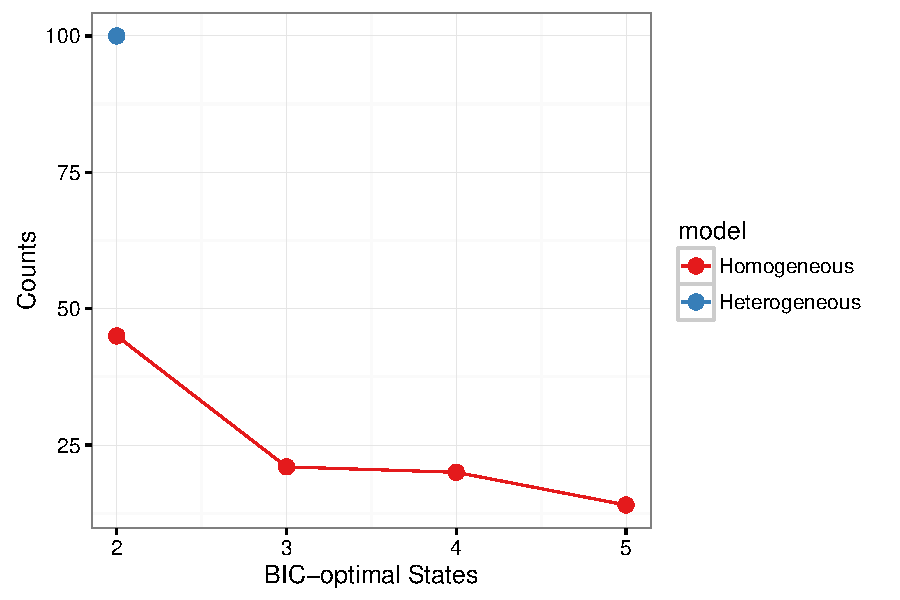
\includegraphics[width=5in]{figure/sim_results-1}
  \caption{\csentence{Simulation Results} BIC-optimal state frequency for 2-6 state HMMs with and without covariate transition on 100 two-state hidden Markov models with covariate transitioning simulations.}
      \end{figure}

\clearpage

  \begin{figure}[h!]
   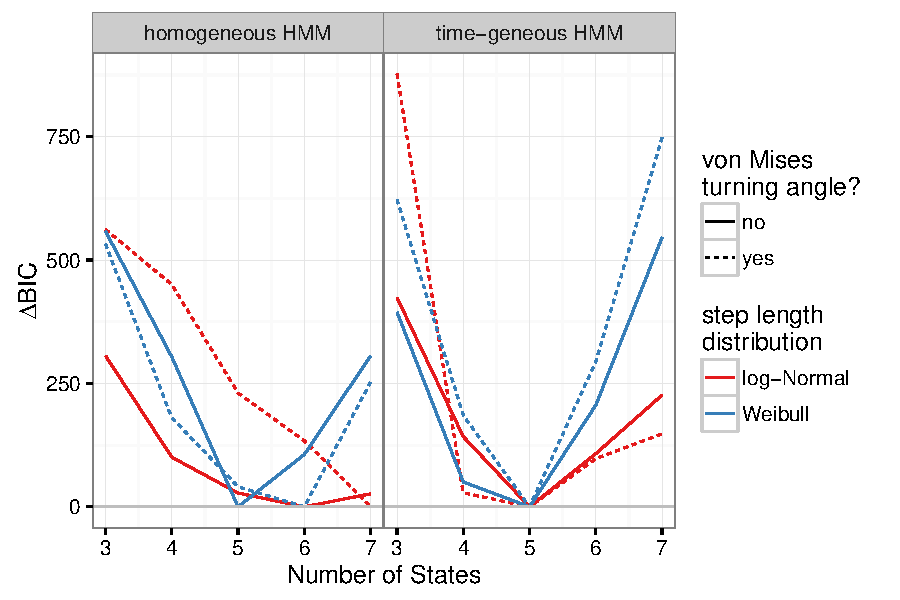
\includegraphics[width=5in]{figure/BICred_plot-1}
  \caption{\csentence{Adjusted BIC Emission Distribution Comparison} Adjusted Bayesian information criterion values for 3-7 state HMMs with different step-length distributions, with and without temporal transitions and turning angles.}
      \end{figure}
      
\clearpage

  \begin{figure}[h!]
   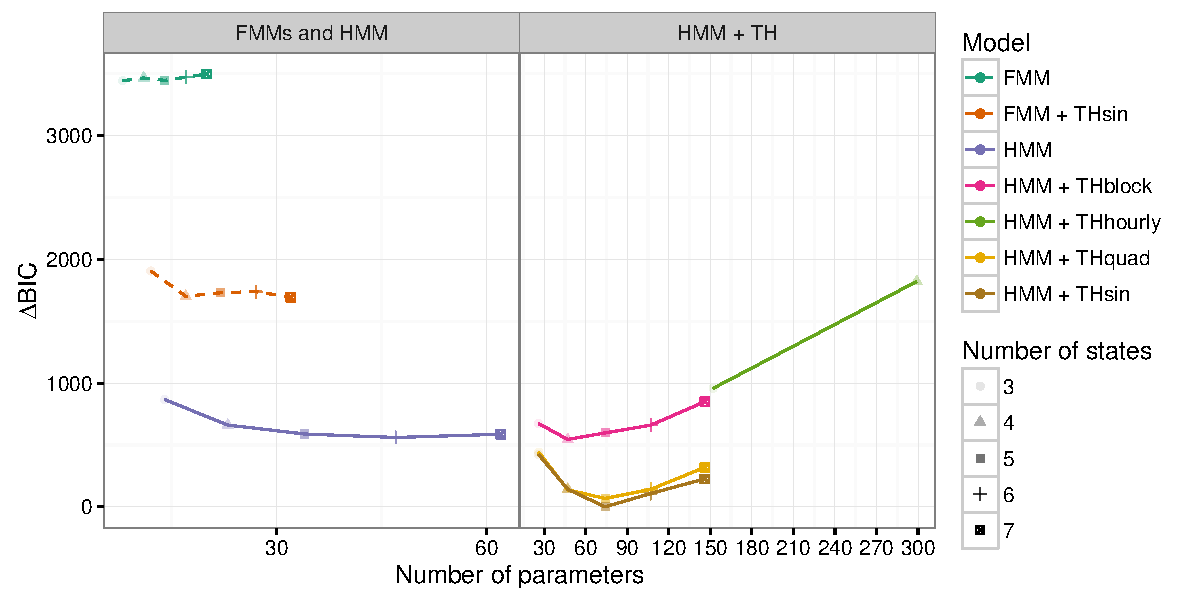
\includegraphics[width=5in]{figure/adj_BIC_comparisons-1}
  \caption{\csentence{Adjusted BICs Across All Models} Adjusted BIC by number of free parameters for HMM model types. The left panel shows homogeneous FMM, heterogeneous FMM (with a sinusoidal prior) and homogeneous HMM. The right panel shows HMMs with different temporal transitions.}
      \end{figure}
      
\clearpage

\begin{figure}[h!]
   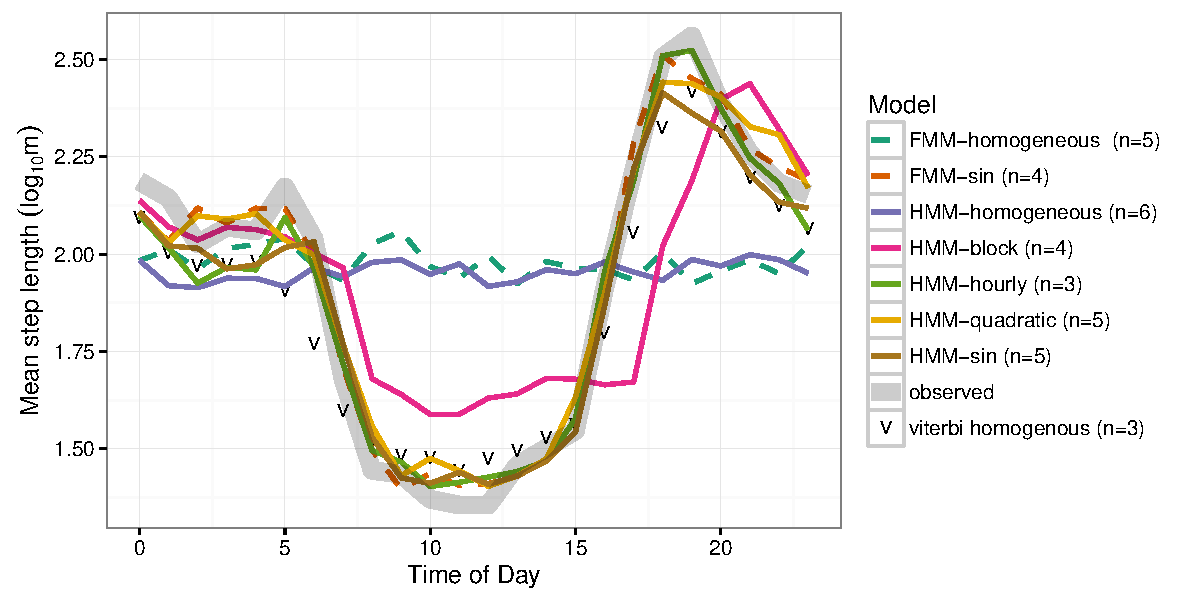
\includegraphics[width=5in]{figure/avg_step_length_by_time-1}
  \caption{\csentence{Diurnal Step Lengths Plot} Average step length by time of day observed (gray highlight), three-state HMM Viterbi predictions (V points), and all transitions type HMMs predictions (out of sample) with their respective BIC-optimal states.}
      \end{figure}
      
\clearpage
      
\begin{figure}[h!]
   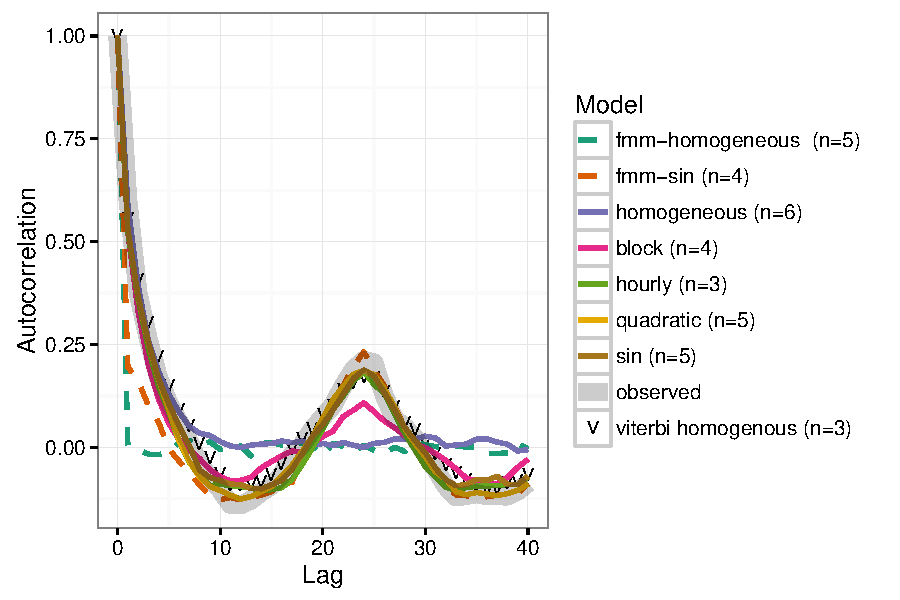
\includegraphics[width=5in]{figure/acf_plot-1}
  \caption{\csentence{Autocorrelation Plot} Autocorrelation of observed (gray highlight), three-state HMM Viterbi predictions (V points), and all transitions type HMMs predictions (out of sample) with their respective BIC-optimal states.}
      \end{figure}
      
\clearpage
      
\begin{figure}[h!]
   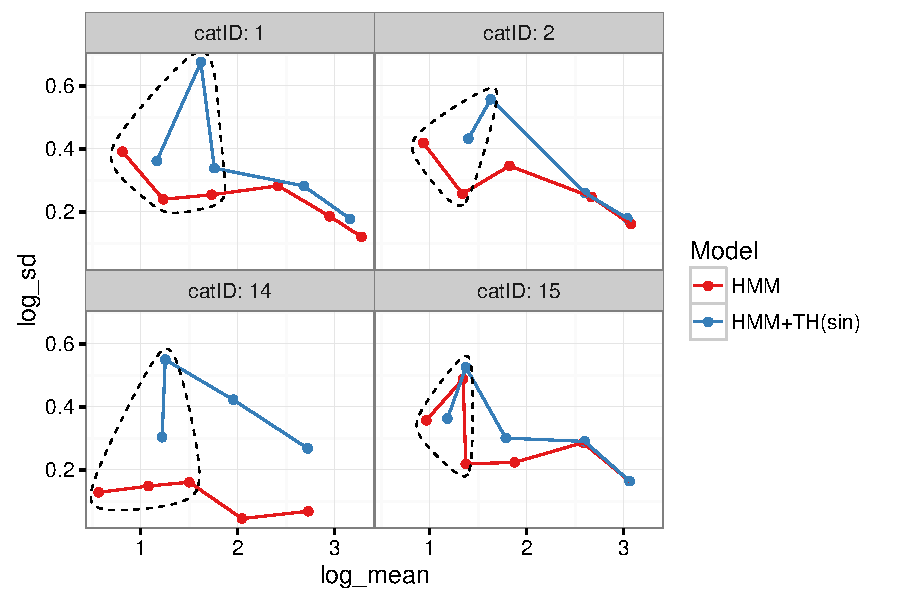
\includegraphics[width=5in]{figure/r_msdlist-1}
  \caption{\csentence{State Identification Plot} Mean and standard deviation of  step length by state for BIC-optimal HMMs (homogeneous and heterogeneous with sinusoidal transition).
      \end{figure}
      
\end{backmatter}
\end{document}
